\subsubsection{UC17 - Visualizzazione avviso: nessuna funzione eseguita}
\begin{figure}[H]
	\centering
	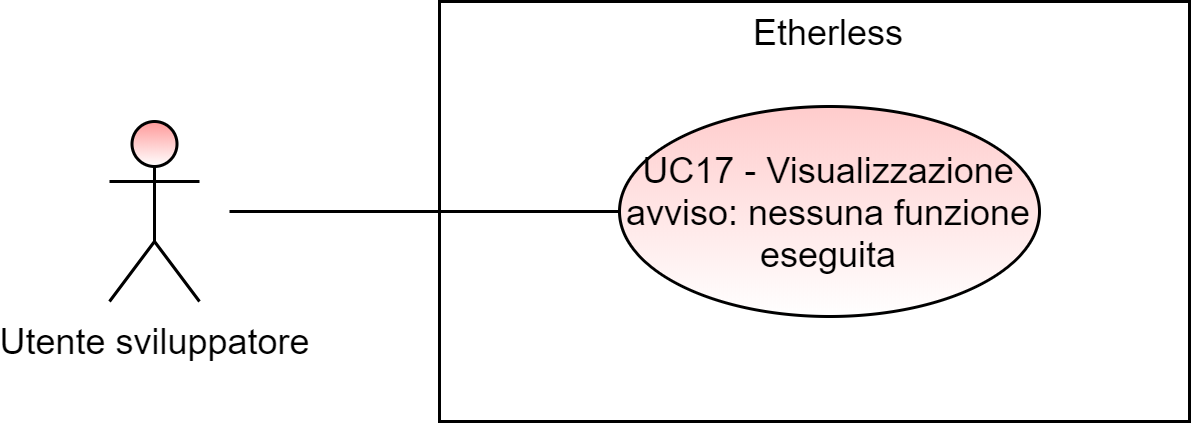
\includegraphics[scale=\ucs]{./res/img/UC17G.png}
	\caption {UC17 - Visualizzazione avviso: nessuna funzione eseguita - schema generale}
\end{figure}
\begin{itemize}
	\item \textbf{Attori primari:} \us{};
	\item \textbf{Descrizione:} l’utente dopo aver eseguito il comando history visualizza un avviso relativo alla mancanza di passate esecuzioni di funzioni all’interno della piattaforma \textit{Etherless};
	\item \textbf{Scenario principale:} 
	\begin{itemize}
		\item l’utente richiede la visualizzazione della propria cronologia di esecuzione tramite il comando \history{};
		\item viene visualizzato un avviso relativo alla mancanza di passate richieste di esecuzione.
	\end{itemize}
	\item \textbf{Precondizione:}  l’utente ha richiesto la visualizzazione della propria cronologia di esecuzione di funzioni non avendo prima eseguito alcuna funzione;
	\item \textbf{Postcondizione:} la CLI\ped{\textit{G}} riporta un avviso che descrive la situazione considerata.  
\end{itemize}